% NOTE: remove [handout] for presentation mode
\documentclass[handout]{beamer}
\usepackage{amsmath}
\usepackage{amssymb}
\usepackage{amsfonts}
\usepackage{subfigure}
\usepackage{algorithm2e}
\usepackage{xspace}
\usepackage{ifthen}
\usepackage{microtype}
\usepackage{color}
\usepackage{bbm}
\usepackage{stmaryrd}
\usepackage{varioref}
\usepackage{natbib}
\bibliographystyle{apalike}

% %
%
%

%
%
\newcommand{\term}[0]{adaptive\xspace}  %
                                %
\newcommand{\Term}[0]{Adaptive\xspace} %

%
%
\newcommand{\citecf}[1]{{\cite<{\cf}, >{#1}}}

%

\newcommand{\certifyingNS}{self--certifying}
\newcommand{\certifying}{self--certifying\xspace}
\newcommand{\Certifying}{Self--Certifying\xspace}

\newcommand{\probname}[0]{Stochastic Submodular Maximization} %

\newcommand{\smushname}[0]{compress\xspace} %
                                %
\newcommand{\AppendixA}[0]{The Appendix\xspace}
%
\newcommand{\appendixA}[0]{the Appendix\xspace}
%


%
%
%
%

%
%
\newcommand{\substitute}[3]{ \ensuremath{{#1}\!\left[{#2}/{#3}\right]} }
\newcommand{\condfun}[2]{\ensuremath{ {#1}^{#2} }}
\newcommand{\averaged}[1]{\ensuremath{#1_{\text{avg}}}} %
                                %
%



%
%
\newcommand{\entropy}[1]{\ensuremath{\mathbb{H}\paren{#1}}}
\newcommand{\infogain}[2]{\ensuremath{\mathbb{I}\paren{{#1} ; {#2}}}}
\newcommand{\support}{\op{support}}
\newcommand{\depth}{\operatorname{depth}} %
\newcommand{\perm}{\operatorname{perm}}   %
\renewcommand{\span}{\operatorname{span}}  
\newcommand{\indicator}[1]{\ensuremath{\one_{#1}}} 
\newcommand{\indicatorset}[1]{\ensuremath{\one_{\set{{#1}}}}} 

\newcommand{\event}[0]{{\mathcal{E}}} 
\newcommand{\instance}[0]{\ensuremath{\mathcal{I}}}

%


%
%
\newcommand {\costminsum}[1]{\ensuremath{c_{\Sigma}\!\paren{#1}}}
\newcommand {\costminsumsym}[0]{\ensuremath{c_{\Sigma}}}
\newcommand{\avgf}[0]{\averaged{f}} %
                                %
\newcommand{\prlzf}[1]{\ensuremath{ f_{\prlz}\!\paren{#1} }}
\newcommand{\prlzfsym}[1]{\ensuremath{ f_{\prlz_{{#1}}} }}
\newcommand{\avgg}[0]{\averaged{g}} %
                                %
\newcommand {\util}[2]{\ensuremath{u\!\paren{{#1}, {#2}}}}
%
%
\newcommand{\avgc}[1]{{c_{\text{avg}}{(#1)}}}
\newcommand{\cavg}[1]{{c_{\text{avg}}{(#1)}}}
\newcommand{\acst}[1]{{c_{\text{avg}}{(#1)}}}
\newcommand{\acstsym}[0]{{c_{\text{avg}}}}
\newcommand{\prlzcst}[2]{{c_{#1}{(#2)}}}
\newcommand{\wcst}[1]{{c_{\text{wc}}{(#1)}}}
\newcommand{\awstsym}[0]{{c_{\text{wc}}}}
\newcommand{\condcost}[2]{\ensuremath{c\paren{ {#2} \! \mid \! {#1} }  }}
%
%
\newcommand{\diff}[2]{\ensuremath{\Delta \hspace{-0.3mm}\paren{ {#2}\! \mid \! {#1} }  }
}  
%

%
%
\newcommand{\sequence}{\sigma}

\newcommand {\Tgreedy}{\ensuremath{T^{\text{greedy}}}}

\newcommand{\policy}[0]{\ensuremath{\pi}}
\newcommand{\greedypolicy}[0]{\ensuremath{\pi^{\text{greedy}}}}
\newcommand{\piavg}{\policy_{\text{avg}}^*}
\newcommand{\policycover}{\policy_{\text{avg}}^*}
\newcommand{\policyproof}{\policy_{\text{proof}}^*}

%
%
\newcommand{\strictprune}[2]{\ensuremath{  #1_{[\gets{#2}] }}} %
\newcommand{\laxprune}[2]{\ensuremath{  #1_{[{#2}\to]}}} %
\newcommand{\prune}[2]{\ensuremath{  #1_{[{#2}]} }  } %
\newcommand{\append}[2]{\ensuremath{{#1}@{#2}}} %

\newcommand{\underTree}[2]{\ensuremath{ #1^{-}_{[#2]}   }} %
\newcommand{\overTree}[2]{\ensuremath{ #1^{+}_{[#2]}   }} %
\newcommand{\treeCov}[3]{\ensuremath{ #1_{[#2] \cup \set{#3}}   }} %
\newcommand{\treeSmush}[3]{\ensuremath{ #1_{[#2] \cup \set{#3}}   }} %
\newcommand{\treeExtend}[3]{\ensuremath{ {#1}\!\# #2_{\set{#3}}   }} %
%

%
%
\newcommand{\node}[0]{\ensuremath{u}}
\newcommand{\elem}[0]{\ensuremath{e}}
\newcommand {\groundset}{\ensuremath{E}} %
\newcommand {\groundsubset}{\ensuremath{A}}%
                                %
\newcommand{\outcome}[0]{\ensuremath{o}} %
\newcommand{\outcomes}[0]{\ensuremath{O}} %
%
\newcommand{\mass}[1]{{\color{black}{\ensuremath{p\paren{#1}}}}}
\newcommand{\rlzmass}[1]{{\color{black}{\ensuremath{p\paren{#1}}}}}
\newcommand{\rlzmasssym}[0]{{\color{black}{\ensuremath{p}}}}
\newcommand{\rlzmassover}[2]{{\color{black}{\ensuremath{p_{#1}\!\paren{#2}}}}}
\newcommand{\rlzprior}[0]{{\color{black}{\ensuremath{p\paren{\rlz}}}}}
\newcommand{\rlz}[0]{{\color{black}{\ensuremath{\phi}}}} %
\newcommand{\rvrlz}[0]{{\color{black}{\ensuremath{\Phi}}}} %
\newcommand{\rlzt}[0]{\ensuremath{\rlz_{\text{true}}}} %
\newcommand{\rvprlz}[0]{{\color{black}{\ensuremath{\Psi}}}} %
\newcommand{\prlz}[0]{{\color{black}{\ensuremath{\psi}}}} %
\newcommand{\prlzsmall}[0]{\ensuremath{\psi}} %

\newcommand{\prlzsub}[2]{\substitute{\prlz}{#1}{#2}}
\newcommand{\prlzeo}[0]{\prlzsub{\elem}{\outcome}}
\newcommand{\prlzxo}[0]{\prlzsub{x}{\outcome}}
%
\newcommand{\vselim}[0]{\ensuremath{\vs_{\text{elim}}}} 

\newcommand{\rlzset}[0]{\mathcal{R}}
\newcommand{\prlzset}[0]{\mathcal{P}}
\newcommand{\htrue}[0]{\ensuremath{h_{\text{true}}}} %
                                %
\newcommand{\itrue}[0]{\ensuremath{i_{\text{true}}}} %
                                %
%



\newcommand{\model}[0]{\ensuremath{\mathcal{M}}}
\newcommand{\distrib}[0]{\ensuremath{\mathcal{D}}}

\newcommand{\quota}[0]{\ensuremath{Q}} %
\newcommand{\budget}[0]{\ensuremath{k}} %
\newcommand{\price}[0]{\ensuremath{\theta}} %
\newcommand{\charge}[1]{\ensuremath{C_{#1}}} %

\newcommand{\progress}[1]{\ensuremath{  \expct{f(\dom({#1}), \rvrlz) \mid
  \rvrlz \sim {#1}}  }}
\newcommand{\progressSet}[2]{\ensuremath{  \expct{f({#1}, \rvrlz) \mid
  \rvrlz \sim {#2}}  }}



%
%
\newcommand{\hypotheses}[0]{\ensuremath{H}} 
\newcommand{\data}[0]{\ensuremath{X}} 
\newcommand{\labels}[0]{\ensuremath{L}} 
\newcommand{\target}[0]{\ensuremath{h^*}} 
\newcommand{\error}[0]{\operatorname{error}} 
\newcommand{\prior}[0]{\ensuremath{p_{\hypotheses}}}
\newcommand{\vs}[0]{\ensuremath{V}\xspace} %
%
 \newcommand{\gbs}[0]{GBS\xspace} %
 \newcommand{\qcost}[2]{\ensuremath{q({#1}, {#2})}} %
\newcommand{\pcost}[2]{\ensuremath{\left\Vert{#1}\right\Vert_{#2}}} %

\newcommand{\ncost}[2]{\ensuremath{c({#1}, {#2})}} %
\newcommand{\vsmass}[2]{\ensuremath{\rho({#1}, {#2})}} %
\newcommand{\pmass}[3]{\ensuremath{\rho({#1}, {#2}; {#3})}} %
                                %
\newcommand{\timetosplit}[1]{\ensuremath{t({#1})}}
\newcommand{\vsmasssymbol}[0]{\ensuremath{\rho}} %
\newcommand{\played}[2]{\groundset({#1}, {#2})} 

\newcommand{\Tgbs}[0]{\ensuremath{T^{\text{GBS}}}} %
                                %
\newcommand{\massleft}[0]{\rho} 
%

\newcommand{\range}[0]{\operatorname{range}} 

\newcommand{\LHS}[1]{\operatorname{LHS}_{#1}}
\newcommand{\RHS}[1]{\operatorname{RHS}_{#1}}

%
%
\newcommand{\partset}[1]{\dot{#1}}
\newcommand{\itemparts}[0]{\partset{\groundset}}
%
%
\newcommand{\prt}[2]{{#1}\!\paren{{#2}}}
\newcommand{\iplayed}[2]{\itemparts({#1}, {#2})} 

%

%
%


\newcommand{\alive}[1]{{A({#1})}} 

%
\newcommand{\EMSE}{EMSE}
\newcommand{\MSE}{MSE}
\newcommand{\numsensors}{\ensuremath{n}}
\newcommand{\fEMSE}{\hat{f}_{\EMSE}}
\newcommand{\sensor}{\ensuremath{v}}
\newcommand{\sensors}{V}
\newcommand{\kernel}{K}
\newcommand{\pfail}[1]{p_{\text{fail}}\!\paren{#1} }

%
\newcommand{\numberof}[0]{\operatorname{rep}}
\newcommand{\invnumberof}[0]{\operatorname{rep}^{-1}}
\newcommand{\nmaps}{m}
\newcommand{\ntreasure}{t}
\newcommand{\nmatrix}{n}
\newcommand{\mapsize}{s}

%
\newcommand{\trace}{\tau}
\newcommand{\ptrace}[2]{\prlz\paren{{#1}, {#2}}}

\newcommand{\leaves}[0]{\mathcal{L}}
\newcommand{\parts}[0]{\mathcal{R}}
\newcommand{\pparts}[0]{\mathcal{P}}

\newcommand{\Xvec}{\mathbf{X}}

\newcommand{\gfloor}{\ensuremath{g^{\floor{k/2}}}}
 
\newcommand{\bound}{\beta}
\newcommand{\avgbound}{\beta_{\text{avg}}}
%

%
%
\newcommand{\daniel}[1]{\ifthenelse{\boolean{showcomments}}{\textcolor{red}{Daniel: #1}}{}}
\newcommand{\andreas}[1]{\ifthenelse{\boolean{showcomments}}{\textcolor{red}{Andreas: #1}}{}}

\newcommand{\myskip}{\myvspace{-0mm}}

\newcommand{\cf}{\emph{c.f.}\xspace}

\newcommand{\captionsmall}[1]{\caption{\small #1}}
\newcommand{\commentout}[1]{}

\newcommand{\family}{{\mathcal{F}}}
\newcommand{\sets}{\ensuremath{\mathcal{S}}}
\newcommand{\collection}{\ensuremath{\mathcal{C}}}

\newcommand{\cS}{{\mathcal{S}}}
\newcommand{\cA}{{\mathcal{A}}}
\newcommand{\cG}{{\mathcal{G}}}
\newcommand{\cE}{{\mathcal{E}}}
\newcommand{\cV}{{\mathcal{V}}}
\newcommand{\cB}{{\mathcal{B}}}
\newcommand{\cX}{{\mathcal{X}}}
\newcommand{\cY}{{\mathcal{Y}}}
\newcommand{\cH}{{\mathcal{H}}}
\newcommand{\cU}{{\mathcal{U}}}
\newcommand{\cW}{{\mathcal{W}}}
\newcommand{\cC}{{\mathcal{C}}}
\newcommand{\cO}{{\mathcal{O}}}

\newcommand{\scen}{{\mathcal{I}}}

\newcommand{\balpha}{{\mathbf{\alpha}}}
\newcommand{\ba}{{\mathbf{a}}}
\newcommand{\bh}{{\mathbf{h}}}
\newcommand{\bs}{{\mathbf{s}}}
\newcommand{\bt}{{\mathbf{t}}}
\newcommand{\bu}{{\mathbf{u}}}
\newcommand{\bv}{{\mathbf{v}}}
\newcommand{\bw}{{\mathbf{w}}}
\newcommand{\bx}{{\mathbf{x}}}
\newcommand{\by}{{\mathbf{y}}}
\newcommand{\bz}{{\mathbf{z}}}


%
%

%
\newlength{\presec}
\newlength{\postsec}
\newlength{\presubsec}
\newlength{\postsubsec}
\newlength{\prepara}
\newlength{\postpara}
\setlength{\presec}{-0mm}
\setlength{\postsec}{-0mm}
\setlength{\presubsec}{-0mm}
\setlength{\postsubsec}{-0mm}
\setlength{\prepara}{-0mm}
\setlength{\postpara}{-0mm}

\newenvironment{Enum}{
\vspace{-0.5em}
\begin{enumerate}
   \setlength{\itemsep}{0.25em}%
  \setlength{\parskip}{0em}
  \setlength{\parsep}{0em}}
{\end{enumerate}\vspace{-0.5em}}

\newcounter{myLISTctr}
\newcommand{\initOneLiners}{%
    \setlength{\itemsep}{0pt}
    \setlength{\parsep }{0pt}
    \setlength{\topsep }{0pt}
%
}
\newenvironment{OneLiners}[1][\ensuremath{\bullet}]
    {\begin{list}
        {#1}
        {\initOneLiners}}
    {\end{list}}


\newenvironment{proofof}[1]{
\noindent{\bf Proof of {#1}:}}
{\hfill$\blacksquare$
}

\newcommand{\ignore}[1]{}

\def \etal {et al.\ }
\def \argmax {\mathop{\rm arg\,max}}
\def \argmin {\mathop{\rm arg\,min}}

\newcommand{\ith}{\ensuremath{i^{\mathrm{th}}}\xspace}
\newcommand{\jth}{\ensuremath{j^{\mathrm{th}}}\xspace}
\newcommand{\op}[1]{\operatorname{#1}}
\newcommand{\one}{\mathbf{1}}
%
\newcommand{\poly}{\operatorname{poly}}
\newcommand{\paren} [1] {\ensuremath{ \left( {#1} \right) }}
\newcommand{\bigparen} [1] {\ensuremath{ \Big( {#1} \Big) }}
%
\renewcommand{\Pr}[1]{\ensuremath{\mathbb{P}\left[#1\right] }}
\newcommand{\prob}[1]{\ensuremath{\mathbb{P}\left[#1\right] }}
\newcommand{\probsym}[0]{\ensuremath{\mathbb{P}}}
\newcommand{\probover}[2]{\ensuremath{\mathbb{P}_{#1}\left[#2\right]
  }}
\newcommand{\proboverrlz}[2]{\ensuremath{\mathbb{P}\left[#2\right] }}
\newcommand{\E}[1]{\ensuremath{\mathbb{E}\left[#1\right] }}
%
\newcommand{\size}[1]{\ensuremath{\left|#1\right|}}
\newcommand{\ceil}[1]{\ensuremath{\left\lceil#1\right\rceil}}
\newcommand{\floor}[1]{\ensuremath{\left\lfloor#1\right\rfloor}}
%
\newcommand{\tuple}[1]{\ensuremath{\langle #1 \rangle}}
\newcommand{\func}[3]{\ensuremath{#1 : #2 \rightarrow #3}}
\newcommand{\problem} [1] {{\sc #1}}
\renewcommand{\implies}[0]{\ensuremath{\Rightarrow}}
%
\newcommand{\PositiveIntegers}{\ensuremath{\mathbb{Z^+}}}
\newcommand{\integers}{\ensuremath{\mathbb{Z}}}
\newcommand{\nats}{\ensuremath{\mathbb{N}}}
\newcommand{\reals}{\ensuremath{\mathbb{R}}}

%
\newcommand{\littleO}[1]{\ensuremath{o\paren{#1}}}
\newcommand{\bigO}[1]{\ensuremath{O\paren{#1}}}
\newcommand{\bigTheta}[1]{\ensuremath{\Theta\paren{#1}}}
\newcommand{\bigOmega}[1]{\ensuremath{\Omega\paren{#1}}}

%
\newcommand{\class} [1] {\textrm{#1}} %
\renewcommand{\P} {\class{P}}
\newcommand{\NP} {\class{NP}}

%

\newcommand{\compactdispmath}[1]{\[ \vspace{-1mm} {#1} \vspace{-0mm}  \]}


%
%
%
%
%
%
\newcommand{\roundindex}{\ensuremath{t}}
\newcommand{\partitionindex}{\ensuremath{k}}

\newcommand{\fullversion}{extended version\xspace}

\newcommand{\features}{\ensuremath{v}}
\newcommand{\NumFeatures}{\ensuremath{m}}
\newcommand{\NumRounds}{\ensuremath{T}}

\newcommand{\colorindex}{\ensuremath{c}}
\newcommand{\Color}{\ensuremath{c}}
\newcommand{\Colors}{\ensuremath{\bracket{\NumColors}}}
\newcommand{\Colorvec}{\ensuremath{ \vec{c} }}

%
\renewcommand{\c}{c}
%
%
%
%
%
%
%
%
%
%
%
%
%
%

%


\newcommand{\assignment}{S}  %
%
%

%


\newcommand {\groundsettimespartitions}{\ensuremath{\groundset\times\bracket{\NumPartitions}}} %
\newcommand {\matroidgroundset}{\ensuremath{\mathcal{X}}}
 %
\newcommand {\listgroundset} {\ensuremath{U}}
\newcommand{\OPT}{\textsf{OPT}}
\newcommand{\NULL}{\textsc{null}}

\newcommand{\obj}{\ensuremath{f}} %

\newcommand{\matroid}{\ensuremath{\mathcal{M}}}

%

\newcommand{\setoflist}[1]{\ensuremath{\operatorname{set}({#1})}}
\newcommand{\listofset}[1]{\ensuremath{\operatorname{list}({#1})}}
\newcommand {\ctr} {click-through-rate\xspace}
\newcommand {\ctrs} {click-through-rates\xspace}

%


%
\newcommand{\omitproof}[1]{}

\newcommand{\bracket}[1]{\left[#1\right]}
\newcommand{\Esub}[2]{\mathbb{E}_{#1}\bracket{#2}}
\newcommand{\sample}{\textsf{sample}}

\newcommand{\Alg}{\ensuremath{\mathcal{A}}}
\newcommand{\AllRows}{\ensuremath{\mathcal{R}_{\bracket{\J}}}}

\newcommand {\feasible} {\mathcal{F}}
\newcommand{\LocallyGreedy}{{\bf LocallyGreedy}\xspace}
\newcommand{\NonNegativeReals}{\ensuremath{\mathbb{R}_{\ge 0}}}
\newcommand{\NonNegativeIntegers}{\ensuremath{\mathbb{Z}_{\ge 0}}}

\newcommand{\NumColors}{\ensuremath{C}}
\newcommand{\NumPartitions}{\ensuremath{K}}
%
\newcommand{\OfflineGreedy}{{\sc TabularGreedy}\xspace}
\newcommand{\OnlineGreedy}{{\sc TGbandit}\xspace}
\newcommand{\Partition}{\ensuremath{P}}
\newcommand{\Regret}{\ensuremath{r}}
\newcommand{\Row}{\ensuremath{R}}
\newcommand{\Rows}{\ensuremath{\mathcal{R}}}
\newcommand{\SubGreedy}{{\bf SubGreedy}\ }



%
\vfuzz2pt %
\hfuzz2pt %
%
%
%
%
%
%
%
%
%
%
%
%
%

%
%
%
%

%
\DeclareMathOperator{\pr}{Pr} \DeclareMathOperator{\dist}{Dist}
\DeclareMathOperator{\dom}{dom}
\newcommand{\expct}[1]{\mathbb{E}\left[#1\right]}
\newcommand{\expctover}[2]{\mathbb{E}_{#1}\!\left[#2\right]}
\newcommand{\expctoverrlz}[2]{\mathbb{E}\left[#2\right]}

\newcommand{\norm}[1]{\left\Vert#1\right\Vert}
\newcommand{\abs}[1]{\left\vert#1\right\vert}
\newcommand{\set}[1]{\left\{#1\right\}}
\newcommand{\Real}{\mathbb R}
\newcommand{\eps}{\varepsilon}
\newcommand{\To}{\longrightarrow}
\newcommand{\BX}{\mathbf{B}(X)}
%
%
%
\DeclareMathOperator{\cP}{P} \DeclareMathOperator{\cNP}{NP}
\DeclareMathOperator{\DTIME}{DTIME}
\newcommand{\maxmarg}{{P}^{max}}

\newcommand{\rew}{\mathfrak{R}}

\newcommand{\hpts}{\hat{p}_{t,\bs}}
\newcommand{\hps}{\hat{p}_\bs}
\newcommand{\hp}{\hat{p}}


%

\newcommand{\denselist}{
    \itemsep -2pt\topsep-8pt\partopsep-8pt
}
\newcommand{\defref}[1]{Definition~\ref{#1}}
\newcommand{\tableref}[1]{Table~\ref{#1}}
\newcommand{\figref}[1]{Fig.~\ref{#1}}
\newcommand{\eqnref}[1]{Eq.~(\ref{#1})}
\newcommand{\secref}[1]{\S\ref{#1}}
\newcommand{\thmref}[1]{Theorem~\ref{#1}}
\newcommand{\corref}[1]{Corollary~\ref{#1}}
\newcommand{\propref}[1]{Proposition~\ref{#1}}
\newcommand{\lemref}[1]{Lemma~\ref{#1}}
\newcommand{\algref}[1]{Algorithm~\ref{#1}}


%
%
%

%
%

%
%
%
%
%
%
%
%
%
%



%
%
%

%
%
\newcommand{\term}[0]{adaptive\xspace}  %
                                %
\newcommand{\Term}[0]{Adaptive\xspace} %

%
%
\newcommand{\citecf}[1]{{\cite<{\cf}, >{#1}}}

%

\newcommand{\certifyingNS}{self--certifying}
\newcommand{\certifying}{self--certifying\xspace}
\newcommand{\Certifying}{Self--Certifying\xspace}

\newcommand{\probname}[0]{Stochastic Submodular Maximization} %

\newcommand{\smushname}[0]{compress\xspace} %
                                %
\newcommand{\AppendixA}[0]{The Appendix\xspace}
%
\newcommand{\appendixA}[0]{the Appendix\xspace}
%


%
%
%
%

%
%
\newcommand{\substitute}[3]{ \ensuremath{{#1}\!\left[{#2}/{#3}\right]} }
\newcommand{\condfun}[2]{\ensuremath{ {#1}^{#2} }}
\newcommand{\averaged}[1]{\ensuremath{#1_{\text{avg}}}} %
                                %
%



%
%
\newcommand{\entropy}[1]{\ensuremath{\mathbb{H}\paren{#1}}}
\newcommand{\infogain}[2]{\ensuremath{\mathbb{I}\paren{{#1} ; {#2}}}}
\newcommand{\support}{\op{support}}
\newcommand{\depth}{\operatorname{depth}} %
\newcommand{\perm}{\operatorname{perm}}   %
\renewcommand{\span}{\operatorname{span}}  
\newcommand{\indicator}[1]{\ensuremath{\one_{#1}}} 
\newcommand{\indicatorset}[1]{\ensuremath{\one_{\set{{#1}}}}} 

\newcommand{\event}[0]{{\mathcal{E}}} 
\newcommand{\instance}[0]{\ensuremath{\mathcal{I}}}

%


%
%
\newcommand {\costminsum}[1]{\ensuremath{c_{\Sigma}\!\paren{#1}}}
\newcommand {\costminsumsym}[0]{\ensuremath{c_{\Sigma}}}
\newcommand{\avgf}[0]{\averaged{f}} %
                                %
\newcommand{\prlzf}[1]{\ensuremath{ f_{\prlz}\!\paren{#1} }}
\newcommand{\prlzfsym}[1]{\ensuremath{ f_{\prlz_{{#1}}} }}
\newcommand{\avgg}[0]{\averaged{g}} %
                                %
\newcommand {\util}[2]{\ensuremath{u\!\paren{{#1}, {#2}}}}
%
%
\newcommand{\avgc}[1]{{c_{\text{avg}}{(#1)}}}
\newcommand{\cavg}[1]{{c_{\text{avg}}{(#1)}}}
\newcommand{\acst}[1]{{c_{\text{avg}}{(#1)}}}
\newcommand{\acstsym}[0]{{c_{\text{avg}}}}
\newcommand{\prlzcst}[2]{{c_{#1}{(#2)}}}
\newcommand{\wcst}[1]{{c_{\text{wc}}{(#1)}}}
\newcommand{\awstsym}[0]{{c_{\text{wc}}}}
\newcommand{\condcost}[2]{\ensuremath{c\paren{ {#2} \! \mid \! {#1} }  }}
%
%
\newcommand{\diff}[2]{\ensuremath{\Delta \hspace{-0.3mm}\paren{ {#2}\! \mid \! {#1} }  }
}  
%

%
%
\newcommand{\sequence}{\sigma}

\newcommand {\Tgreedy}{\ensuremath{T^{\text{greedy}}}}

\newcommand{\policy}[0]{\ensuremath{\pi}}
\newcommand{\greedypolicy}[0]{\ensuremath{\pi^{\text{greedy}}}}
\newcommand{\piavg}{\policy_{\text{avg}}^*}
\newcommand{\policycover}{\policy_{\text{avg}}^*}
\newcommand{\policyproof}{\policy_{\text{proof}}^*}

%
%
\newcommand{\strictprune}[2]{\ensuremath{  #1_{[\gets{#2}] }}} %
\newcommand{\laxprune}[2]{\ensuremath{  #1_{[{#2}\to]}}} %
\newcommand{\prune}[2]{\ensuremath{  #1_{[{#2}]} }  } %
\newcommand{\append}[2]{\ensuremath{{#1}@{#2}}} %

\newcommand{\underTree}[2]{\ensuremath{ #1^{-}_{[#2]}   }} %
\newcommand{\overTree}[2]{\ensuremath{ #1^{+}_{[#2]}   }} %
\newcommand{\treeCov}[3]{\ensuremath{ #1_{[#2] \cup \set{#3}}   }} %
\newcommand{\treeSmush}[3]{\ensuremath{ #1_{[#2] \cup \set{#3}}   }} %
\newcommand{\treeExtend}[3]{\ensuremath{ {#1}\!\# #2_{\set{#3}}   }} %
%

%
%
\newcommand{\node}[0]{\ensuremath{u}}
\newcommand{\elem}[0]{\ensuremath{e}}
\newcommand {\groundset}{\ensuremath{E}} %
\newcommand {\groundsubset}{\ensuremath{A}}%
                                %
\newcommand{\outcome}[0]{\ensuremath{o}} %
\newcommand{\outcomes}[0]{\ensuremath{O}} %
%
\newcommand{\mass}[1]{{\color{black}{\ensuremath{p\paren{#1}}}}}
\newcommand{\rlzmass}[1]{{\color{black}{\ensuremath{p\paren{#1}}}}}
\newcommand{\rlzmasssym}[0]{{\color{black}{\ensuremath{p}}}}
\newcommand{\rlzmassover}[2]{{\color{black}{\ensuremath{p_{#1}\!\paren{#2}}}}}
\newcommand{\rlzprior}[0]{{\color{black}{\ensuremath{p\paren{\rlz}}}}}
\newcommand{\rlz}[0]{{\color{black}{\ensuremath{\phi}}}} %
\newcommand{\rvrlz}[0]{{\color{black}{\ensuremath{\Phi}}}} %
\newcommand{\rlzt}[0]{\ensuremath{\rlz_{\text{true}}}} %
\newcommand{\rvprlz}[0]{{\color{black}{\ensuremath{\Psi}}}} %
\newcommand{\prlz}[0]{{\color{black}{\ensuremath{\psi}}}} %
\newcommand{\prlzsmall}[0]{\ensuremath{\psi}} %

\newcommand{\prlzsub}[2]{\substitute{\prlz}{#1}{#2}}
\newcommand{\prlzeo}[0]{\prlzsub{\elem}{\outcome}}
\newcommand{\prlzxo}[0]{\prlzsub{x}{\outcome}}
%
\newcommand{\vselim}[0]{\ensuremath{\vs_{\text{elim}}}} 

\newcommand{\rlzset}[0]{\mathcal{R}}
\newcommand{\prlzset}[0]{\mathcal{P}}
\newcommand{\htrue}[0]{\ensuremath{h_{\text{true}}}} %
                                %
\newcommand{\itrue}[0]{\ensuremath{i_{\text{true}}}} %
                                %
%



\newcommand{\model}[0]{\ensuremath{\mathcal{M}}}
\newcommand{\distrib}[0]{\ensuremath{\mathcal{D}}}

\newcommand{\quota}[0]{\ensuremath{Q}} %
\newcommand{\budget}[0]{\ensuremath{k}} %
\newcommand{\price}[0]{\ensuremath{\theta}} %
\newcommand{\charge}[1]{\ensuremath{C_{#1}}} %

\newcommand{\progress}[1]{\ensuremath{  \expct{f(\dom({#1}), \rvrlz) \mid
  \rvrlz \sim {#1}}  }}
\newcommand{\progressSet}[2]{\ensuremath{  \expct{f({#1}, \rvrlz) \mid
  \rvrlz \sim {#2}}  }}



%
%
\newcommand{\hypotheses}[0]{\ensuremath{H}} 
\newcommand{\data}[0]{\ensuremath{X}} 
\newcommand{\labels}[0]{\ensuremath{L}} 
\newcommand{\target}[0]{\ensuremath{h^*}} 
\newcommand{\error}[0]{\operatorname{error}} 
\newcommand{\prior}[0]{\ensuremath{p_{\hypotheses}}}
\newcommand{\vs}[0]{\ensuremath{V}\xspace} %
%
 \newcommand{\gbs}[0]{GBS\xspace} %
 \newcommand{\qcost}[2]{\ensuremath{q({#1}, {#2})}} %
\newcommand{\pcost}[2]{\ensuremath{\left\Vert{#1}\right\Vert_{#2}}} %

\newcommand{\ncost}[2]{\ensuremath{c({#1}, {#2})}} %
\newcommand{\vsmass}[2]{\ensuremath{\rho({#1}, {#2})}} %
\newcommand{\pmass}[3]{\ensuremath{\rho({#1}, {#2}; {#3})}} %
                                %
\newcommand{\timetosplit}[1]{\ensuremath{t({#1})}}
\newcommand{\vsmasssymbol}[0]{\ensuremath{\rho}} %
\newcommand{\played}[2]{\groundset({#1}, {#2})} 

\newcommand{\Tgbs}[0]{\ensuremath{T^{\text{GBS}}}} %
                                %
\newcommand{\massleft}[0]{\rho} 
%

\newcommand{\range}[0]{\operatorname{range}} 

\newcommand{\LHS}[1]{\operatorname{LHS}_{#1}}
\newcommand{\RHS}[1]{\operatorname{RHS}_{#1}}

%
%
\newcommand{\partset}[1]{\dot{#1}}
\newcommand{\itemparts}[0]{\partset{\groundset}}
%
%
\newcommand{\prt}[2]{{#1}\!\paren{{#2}}}
\newcommand{\iplayed}[2]{\itemparts({#1}, {#2})} 

%

%
%


\newcommand{\alive}[1]{{A({#1})}} 

%
\newcommand{\EMSE}{EMSE}
\newcommand{\MSE}{MSE}
\newcommand{\numsensors}{\ensuremath{n}}
\newcommand{\fEMSE}{\hat{f}_{\EMSE}}
\newcommand{\sensor}{\ensuremath{v}}
\newcommand{\sensors}{V}
\newcommand{\kernel}{K}
\newcommand{\pfail}[1]{p_{\text{fail}}\!\paren{#1} }

%
\newcommand{\numberof}[0]{\operatorname{rep}}
\newcommand{\invnumberof}[0]{\operatorname{rep}^{-1}}
\newcommand{\nmaps}{m}
\newcommand{\ntreasure}{t}
\newcommand{\nmatrix}{n}
\newcommand{\mapsize}{s}

%
\newcommand{\trace}{\tau}
\newcommand{\ptrace}[2]{\prlz\paren{{#1}, {#2}}}

\newcommand{\leaves}[0]{\mathcal{L}}
\newcommand{\parts}[0]{\mathcal{R}}
\newcommand{\pparts}[0]{\mathcal{P}}

\newcommand{\Xvec}{\mathbf{X}}

\newcommand{\gfloor}{\ensuremath{g^{\floor{k/2}}}}
 
\newcommand{\bound}{\beta}
\newcommand{\avgbound}{\beta_{\text{avg}}}
%

%
%
\newcommand{\daniel}[1]{\ifthenelse{\boolean{showcomments}}{\textcolor{red}{Daniel: #1}}{}}
\newcommand{\andreas}[1]{\ifthenelse{\boolean{showcomments}}{\textcolor{red}{Andreas: #1}}{}}

\newcommand{\myskip}{\myvspace{-0mm}}

\newcommand{\cf}{\emph{c.f.}\xspace}

\newcommand{\captionsmall}[1]{\caption{\small #1}}
\newcommand{\commentout}[1]{}

\newcommand{\family}{{\mathcal{F}}}
\newcommand{\sets}{\ensuremath{\mathcal{S}}}
\newcommand{\collection}{\ensuremath{\mathcal{C}}}

\newcommand{\cS}{{\mathcal{S}}}
\newcommand{\cA}{{\mathcal{A}}}
\newcommand{\cG}{{\mathcal{G}}}
\newcommand{\cE}{{\mathcal{E}}}
\newcommand{\cV}{{\mathcal{V}}}
\newcommand{\cB}{{\mathcal{B}}}
\newcommand{\cX}{{\mathcal{X}}}
\newcommand{\cY}{{\mathcal{Y}}}
\newcommand{\cH}{{\mathcal{H}}}
\newcommand{\cU}{{\mathcal{U}}}
\newcommand{\cW}{{\mathcal{W}}}
\newcommand{\cC}{{\mathcal{C}}}
\newcommand{\cO}{{\mathcal{O}}}

\newcommand{\scen}{{\mathcal{I}}}

\newcommand{\balpha}{{\mathbf{\alpha}}}
\newcommand{\ba}{{\mathbf{a}}}
\newcommand{\bh}{{\mathbf{h}}}
\newcommand{\bs}{{\mathbf{s}}}
\newcommand{\bt}{{\mathbf{t}}}
\newcommand{\bu}{{\mathbf{u}}}
\newcommand{\bv}{{\mathbf{v}}}
\newcommand{\bw}{{\mathbf{w}}}
\newcommand{\bx}{{\mathbf{x}}}
\newcommand{\by}{{\mathbf{y}}}
\newcommand{\bz}{{\mathbf{z}}}


%
%

%
\newlength{\presec}
\newlength{\postsec}
\newlength{\presubsec}
\newlength{\postsubsec}
\newlength{\prepara}
\newlength{\postpara}
\setlength{\presec}{-0mm}
\setlength{\postsec}{-0mm}
\setlength{\presubsec}{-0mm}
\setlength{\postsubsec}{-0mm}
\setlength{\prepara}{-0mm}
\setlength{\postpara}{-0mm}

\newenvironment{Enum}{
\vspace{-0.5em}
\begin{enumerate}
   \setlength{\itemsep}{0.25em}%
  \setlength{\parskip}{0em}
  \setlength{\parsep}{0em}}
{\end{enumerate}\vspace{-0.5em}}

\newcounter{myLISTctr}
\newcommand{\initOneLiners}{%
    \setlength{\itemsep}{0pt}
    \setlength{\parsep }{0pt}
    \setlength{\topsep }{0pt}
%
}
\newenvironment{OneLiners}[1][\ensuremath{\bullet}]
    {\begin{list}
        {#1}
        {\initOneLiners}}
    {\end{list}}


\newenvironment{proofof}[1]{
\noindent{\bf Proof of {#1}:}}
{\hfill$\blacksquare$
}

\newcommand{\ignore}[1]{}

\def \etal {et al.\ }
\def \argmax {\mathop{\rm arg\,max}}
\def \argmin {\mathop{\rm arg\,min}}

\newcommand{\ith}{\ensuremath{i^{\mathrm{th}}}\xspace}
\newcommand{\jth}{\ensuremath{j^{\mathrm{th}}}\xspace}
\newcommand{\op}[1]{\operatorname{#1}}
\newcommand{\one}{\mathbf{1}}
%
\newcommand{\poly}{\operatorname{poly}}
\newcommand{\paren} [1] {\ensuremath{ \left( {#1} \right) }}
\newcommand{\bigparen} [1] {\ensuremath{ \Big( {#1} \Big) }}
%
\renewcommand{\Pr}[1]{\ensuremath{\mathbb{P}\left[#1\right] }}
\newcommand{\prob}[1]{\ensuremath{\mathbb{P}\left[#1\right] }}
\newcommand{\probsym}[0]{\ensuremath{\mathbb{P}}}
\newcommand{\probover}[2]{\ensuremath{\mathbb{P}_{#1}\left[#2\right]
  }}
\newcommand{\proboverrlz}[2]{\ensuremath{\mathbb{P}\left[#2\right] }}
\newcommand{\E}[1]{\ensuremath{\mathbb{E}\left[#1\right] }}
%
\newcommand{\size}[1]{\ensuremath{\left|#1\right|}}
\newcommand{\ceil}[1]{\ensuremath{\left\lceil#1\right\rceil}}
\newcommand{\floor}[1]{\ensuremath{\left\lfloor#1\right\rfloor}}
%
\newcommand{\tuple}[1]{\ensuremath{\langle #1 \rangle}}
\newcommand{\func}[3]{\ensuremath{#1 : #2 \rightarrow #3}}
\newcommand{\problem} [1] {{\sc #1}}
\renewcommand{\implies}[0]{\ensuremath{\Rightarrow}}
%
\newcommand{\PositiveIntegers}{\ensuremath{\mathbb{Z^+}}}
\newcommand{\integers}{\ensuremath{\mathbb{Z}}}
\newcommand{\nats}{\ensuremath{\mathbb{N}}}
\newcommand{\reals}{\ensuremath{\mathbb{R}}}

%
\newcommand{\littleO}[1]{\ensuremath{o\paren{#1}}}
\newcommand{\bigO}[1]{\ensuremath{O\paren{#1}}}
\newcommand{\bigTheta}[1]{\ensuremath{\Theta\paren{#1}}}
\newcommand{\bigOmega}[1]{\ensuremath{\Omega\paren{#1}}}

%
\newcommand{\class} [1] {\textrm{#1}} %
\renewcommand{\P} {\class{P}}
\newcommand{\NP} {\class{NP}}

%

\newcommand{\compactdispmath}[1]{\[ \vspace{-1mm} {#1} \vspace{-0mm}  \]}


%
%
%
%
%
%
\newcommand{\roundindex}{\ensuremath{t}}
\newcommand{\partitionindex}{\ensuremath{k}}

\newcommand{\fullversion}{extended version\xspace}

\newcommand{\features}{\ensuremath{v}}
\newcommand{\NumFeatures}{\ensuremath{m}}
\newcommand{\NumRounds}{\ensuremath{T}}

\newcommand{\colorindex}{\ensuremath{c}}
\newcommand{\Color}{\ensuremath{c}}
\newcommand{\Colors}{\ensuremath{\bracket{\NumColors}}}
\newcommand{\Colorvec}{\ensuremath{ \vec{c} }}

%
\renewcommand{\c}{c}
%
%
%
%
%
%
%
%
%
%
%
%
%
%

%


\newcommand{\assignment}{S}  %
%
%

%


\newcommand {\groundsettimespartitions}{\ensuremath{\groundset\times\bracket{\NumPartitions}}} %
\newcommand {\matroidgroundset}{\ensuremath{\mathcal{X}}}
 %
\newcommand {\listgroundset} {\ensuremath{U}}
\newcommand{\OPT}{\textsf{OPT}}
\newcommand{\NULL}{\textsc{null}}

\newcommand{\obj}{\ensuremath{f}} %

\newcommand{\matroid}{\ensuremath{\mathcal{M}}}

%

\newcommand{\setoflist}[1]{\ensuremath{\operatorname{set}({#1})}}
\newcommand{\listofset}[1]{\ensuremath{\operatorname{list}({#1})}}
\newcommand {\ctr} {click-through-rate\xspace}
\newcommand {\ctrs} {click-through-rates\xspace}

%


%
\newcommand{\omitproof}[1]{}

\newcommand{\bracket}[1]{\left[#1\right]}
\newcommand{\Esub}[2]{\mathbb{E}_{#1}\bracket{#2}}
\newcommand{\sample}{\textsf{sample}}

\newcommand{\Alg}{\ensuremath{\mathcal{A}}}
\newcommand{\AllRows}{\ensuremath{\mathcal{R}_{\bracket{\J}}}}

\newcommand {\feasible} {\mathcal{F}}
\newcommand{\LocallyGreedy}{{\bf LocallyGreedy}\xspace}
\newcommand{\NonNegativeReals}{\ensuremath{\mathbb{R}_{\ge 0}}}
\newcommand{\NonNegativeIntegers}{\ensuremath{\mathbb{Z}_{\ge 0}}}

\newcommand{\NumColors}{\ensuremath{C}}
\newcommand{\NumPartitions}{\ensuremath{K}}
%
\newcommand{\OfflineGreedy}{{\sc TabularGreedy}\xspace}
\newcommand{\OnlineGreedy}{{\sc TGbandit}\xspace}
\newcommand{\Partition}{\ensuremath{P}}
\newcommand{\Regret}{\ensuremath{r}}
\newcommand{\Row}{\ensuremath{R}}
\newcommand{\Rows}{\ensuremath{\mathcal{R}}}
\newcommand{\SubGreedy}{{\bf SubGreedy}\ }



%
\vfuzz2pt %
\hfuzz2pt %
%
%
%
%
%
%
%
%
%
%
%
%
%

%
%
%
%

%
\DeclareMathOperator{\pr}{Pr} \DeclareMathOperator{\dist}{Dist}
\DeclareMathOperator{\dom}{dom}
\newcommand{\expct}[1]{\mathbb{E}\left[#1\right]}
\newcommand{\expctover}[2]{\mathbb{E}_{#1}\!\left[#2\right]}
\newcommand{\expctoverrlz}[2]{\mathbb{E}\left[#2\right]}

\newcommand{\norm}[1]{\left\Vert#1\right\Vert}
\newcommand{\abs}[1]{\left\vert#1\right\vert}
\newcommand{\set}[1]{\left\{#1\right\}}
\newcommand{\Real}{\mathbb R}
\newcommand{\eps}{\varepsilon}
\newcommand{\To}{\longrightarrow}
\newcommand{\BX}{\mathbf{B}(X)}
%
%
%
\DeclareMathOperator{\cP}{P} \DeclareMathOperator{\cNP}{NP}
\DeclareMathOperator{\DTIME}{DTIME}
\newcommand{\maxmarg}{{P}^{max}}

\newcommand{\rew}{\mathfrak{R}}

\newcommand{\hpts}{\hat{p}_{t,\bs}}
\newcommand{\hps}{\hat{p}_\bs}
\newcommand{\hp}{\hat{p}}


%

\newcommand{\denselist}{
    \itemsep -2pt\topsep-8pt\partopsep-8pt
}
\newcommand{\defref}[1]{Definition~\ref{#1}}
\newcommand{\tableref}[1]{Table~\ref{#1}}
\newcommand{\figref}[1]{Fig.~\ref{#1}}
\newcommand{\eqnref}[1]{Eq.~(\ref{#1})}
\newcommand{\secref}[1]{\S\ref{#1}}
\newcommand{\thmref}[1]{Theorem~\ref{#1}}
\newcommand{\corref}[1]{Corollary~\ref{#1}}
\newcommand{\propref}[1]{Proposition~\ref{#1}}
\newcommand{\lemref}[1]{Lemma~\ref{#1}}
\newcommand{\algref}[1]{Algorithm~\ref{#1}}


%
%
%

%
%

%
%
%
%
%
%
%
%
%
%




% Use a clean theme with a sidebar.
\usetheme{Goettingen}
\usecolortheme{dove}
\setbeamercovered{transparent}

\begin{document}

%% Title and ToC
\title[Adaptive Submodularity]{Adaptive Submodularity\\for Active Classification}
\author[]{Sergey Karayev}
\date[Dec 2013]{December 2013\\CS 270 Project}
\frame{
    \titlepage
}

\begin{frame}\frametitle{Table of Contents}
\tableofcontents[]
\end{frame}


%% Introduction
\section{Problem}

\begin{frame}\frametitle{Problem}
\begin{itemize}
    \item Have:
        \begin{itemize}
            \item Hypothesis $H \in \mathcal{H}$, set of possible observations $\mathcal{X} = \{X_1, \dots, X_F\}$.
            \item Each $X_i$ has cost $c_i$ and depends on $H$ in some way.
        \end{itemize}
    \pause
    \item Goal: select subset $\mathcal{X}_S$ to maximize reward $f(\mathcal{X}_S)$.
    \begin{itemize}
        % \item For example, decision theoretic: $f(H, \mathcal{X}_S) = \max_a \sum_h P(h \mid \mathcal{X}_S) U(h, a)$.
        \item e.g. loss: $f(\mathcal{X}_S) = -\ell(h^*, \argmax_h P(h \mid \mathcal{X}_S))$.
        \item e.g. entropy: $f(\mathcal{X}_S) = \sum_x P(h \mid \mathcal{X}_S) \log P(h \mid \mathcal{X}_S)$
    \end{itemize}
    \pause
    \item Variants:
    \begin{itemize}
        \item \emph{Budgeted maximization}: Maximize objective without exceeding cost budget.
        \item \emph{Minimum-cost cover}: Minimize cost while achieving some minimum objective value.
    \end{itemize}
\end{itemize}
\end{frame}

\begin{frame}\frametitle{Active classification}
\begin{itemize}
    \item Furthermore, want to do this \emph{adaptively}: selecting and observing values in sequence (motivation to follow).
    \pause
    \item Lots of recent work in this setting: POMDPs, cascades, trees for spam detection, object recognition, sentence parsing.
    \pause
    \item Different heuristic methods, but no performance guarantees.
    \pause
    \item Here, we synthesize a few recent papers that may construe a promising avenue for theoretical analysis of the active classification problem.
\end{itemize}
\end{frame}


%% Solving offline with submodularity.
\section{Offline solution}

\begin{frame}\frametitle{Offline problem formulation}
Take the problem of selecting the whole subset before observing anything; assume uniform costs.
\vfill
\pause
\begin{columns}[c]
\column{.5\linewidth}
    \centering
    \underline{Budgeted maximization}
    \begin{align*}
    &\underset{\mathcal{X}_S \subseteq \mathcal{X}}{\argmax}\ f(\mathcal{X}_S)\\
    s.t &\ |\mathcal{X}_S| \leq N
    \end{align*}

\column{.5\linewidth}
    \centering
    \underline{Min-cost cover}
    \begin{align*}
    &\underset{\mathcal{X}_S \subseteq \mathcal{X}}{\argmin}\ |\mathcal{X}_S|\\
    s.t &\ f(\mathcal{X}_S) \geq Q
    \end{align*}
\end{columns}
\vfill
\begin{itemize}
    \pause
    \item For most interesting $f$, this is NP-hard.
    \pause
    \item \cite{Nemhauser-1978} showed that if $f$ is \emph{monotone submodular}, then a simple greedy algorithm is near-optimal with these bounds:
\end{itemize}

\visible<4->{
    \begin{columns}[c]
    \column{.5\linewidth}
    \centering
    $$f(\mathcal{X}_{S_N}) \geq (1-\frac{1}{e})\, f(\mathcal{X}_{S_N}^*)$$
    % the greedy solution is at least 63% as good as optimal.
    \column{.5\linewidth}
    \centering
    $$|\mathcal{X}_{S_Q}| \leq |\mathcal{X}_S^*|\, (1 + \log \max_X f(X))$$
    % the greedy solution is at most a logarithmic factor larger than the min cost solution.
    \end{columns}
}

\end{frame}

\subsection{Submodular functions}

\begin{frame}\frametitle{Monotone submodular functions}
\begin{itemize}
    \item Intuitively, submodularity is the property of diminishing returns. For proving near-optimality of the greedy method, we additionally require monotonicity.
    \pause
    \item Define the \emph{gain} of adding another item to a set as $$\Delta_f(X \mid \mathcal{X}_A) = f(\mathcal{X}_A \cup \{X\}) - f(\mathcal{X}_A)$$
    \pause
    \item For all $X$, the submodularity requirement must hold. ``Adding an element to a smaller set helps more than adding the same element to a larger set.''
$$\mathcal{X}_A \subseteq \mathcal{X}_B \implies \Delta_f(X \mid \mathcal{X}_A) \geq \Delta_f(X \mid \mathcal{X}_B)$$
    \pause
    \item For all $X$, the monotonicity requirement must hold. ``Adding an element can never hurt.''
$$\Delta_f(X \mid \mathcal{X}_A) \geq 0$$
\end{itemize}
\end{frame}

\subsection{Greedy algorithm}

\begin{frame}\frametitle{Greedy algorithm}
\vspace{1em}
\begin{algorithm}[H]
\KwIn{Budget $N$; observations $\mathcal{X}$; objective $f$.}
\KwOut{Set $\groundsubset \subseteq \groundset$ of size $N$}
\Begin{
    $\groundsubset\leftarrow\emptyset$\;
    \For{$i=1$ \KwTo $k$}{
        \lForEach{$\elem\in\groundset\setminus \groundsubset$}{compute $\Delta_f(\elem \mid \mathcal{X}_S)$}
        Select $X^* \in \underset{X}{\argmax} \frac{\Delta_f(\elem \mid \mathcal{X}_S)}{c(X)}$\;
        Set $\groundsubset \leftarrow \groundsubset \cup \{\elem^{*}\}$\;
    }
}
\end{algorithm}
\pause
\begin{itemize}
\item Costs have been omitted in the exposition, but are handled by the algorithm if the cost function is modular: $$c(\mathcal{X}_S) = \sum_{X \in \mathcal{X}_S} c(X)$$.
\end{itemize}
\end{frame}

\subsection{Example}

\begin{frame}\frametitle{Example}
\centering
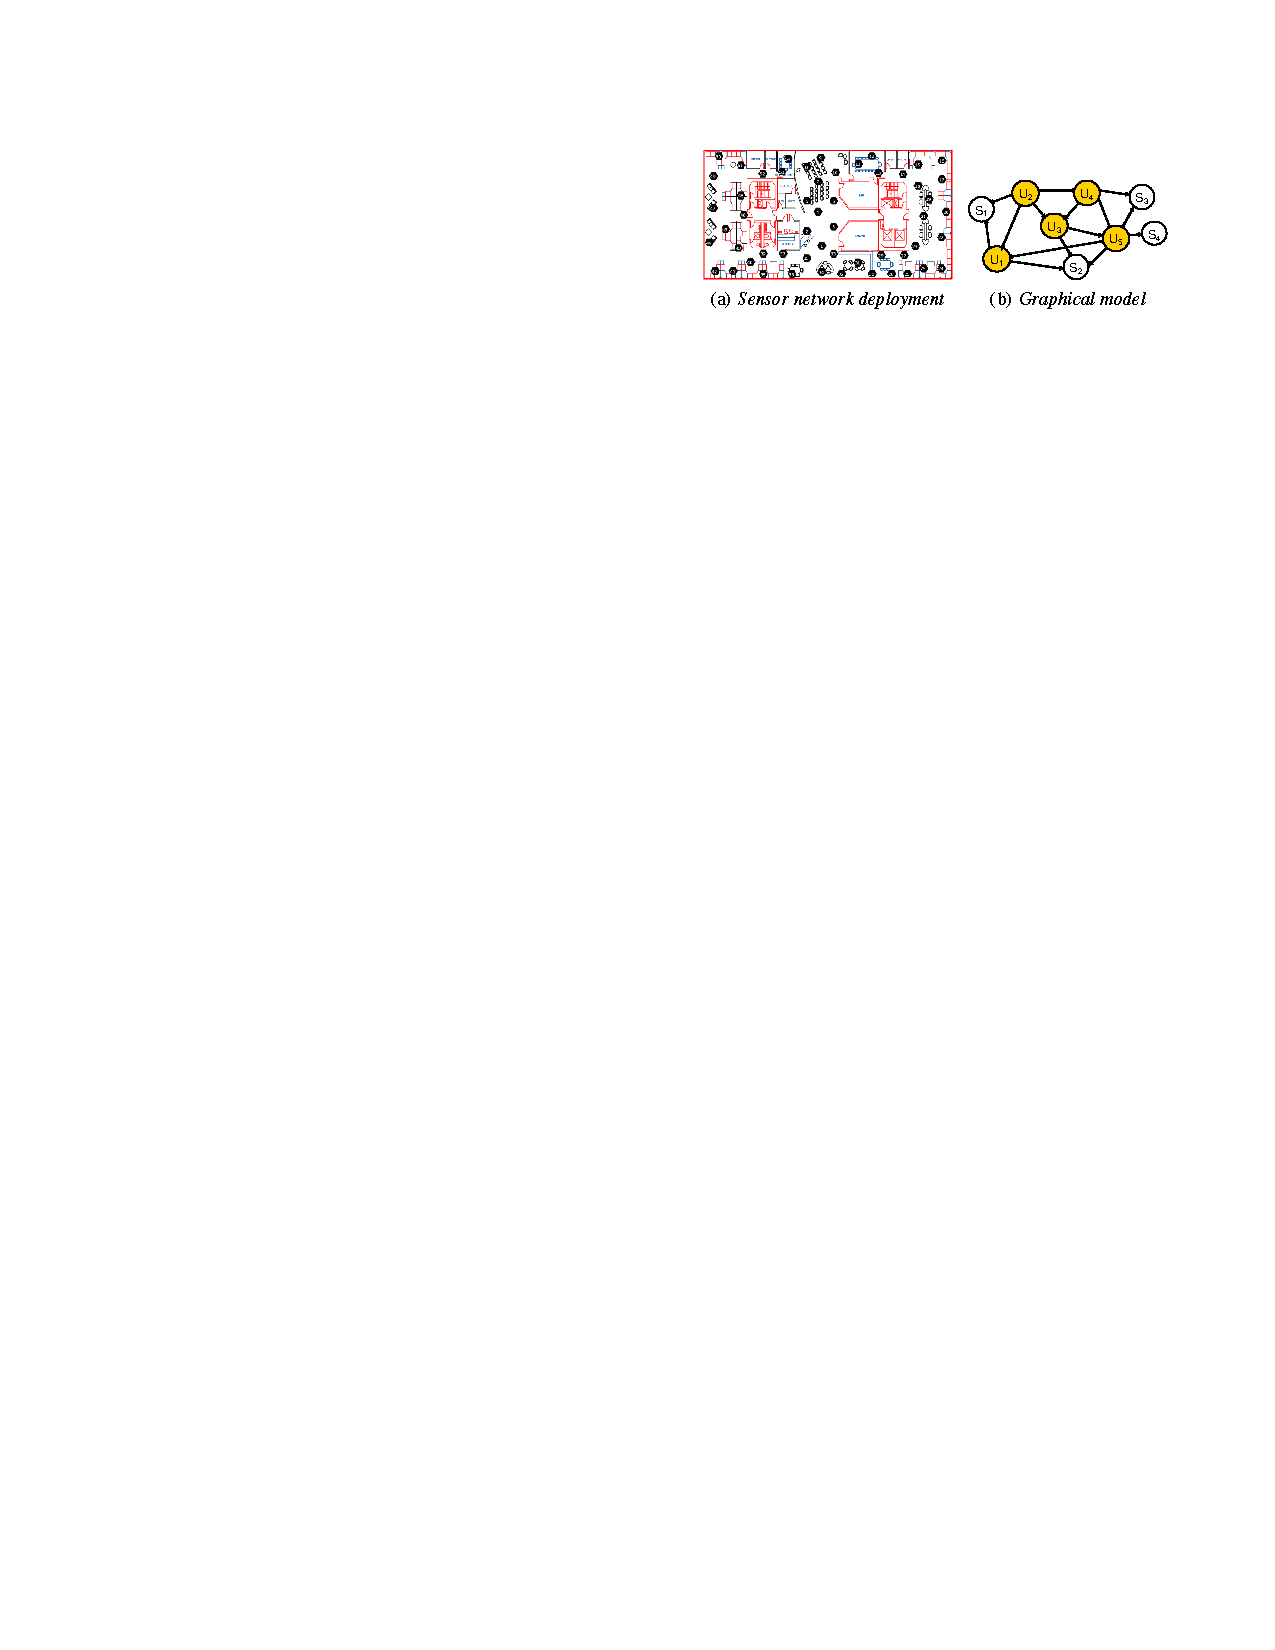
\includegraphics[width=0.8\linewidth]{../figures/sensor.pdf}
\begin{itemize}
    \item Sensor network: want minimal set of observations (Sensors) to maximize utility over  hidden variables (Fire): f(P(Fire $\mid$ Sensors)).
    \pause
    \item If the observation model satisfies certain conditional independence requirements, then Information Gain (reduction in entropy) is submodular [\cite{Krause-UAI-2005}].
    \pause
    \item Classification models like Naive Bayes are very similar.
\end{itemize}
\end{frame}


%% Solving online with adaptive submodularity.
\section{Adaptive solution}

\subsection{Motivation}

\begin{frame}\frametitle{Adaptivity motivation}
\begin{itemize}
    \item With the greedy algorithm and monotone submodular objective, we can find a near-optimal subset.
    \pause
    \item But what if we can observe the results of our actions upon execution?
    \pause
    \item In this case, offline submodularity also can be exponentially far from optimal [\cite{DBLP:journals/corr/abs-1106-5829}].
\end{itemize}
\centering
\visible<3>{
    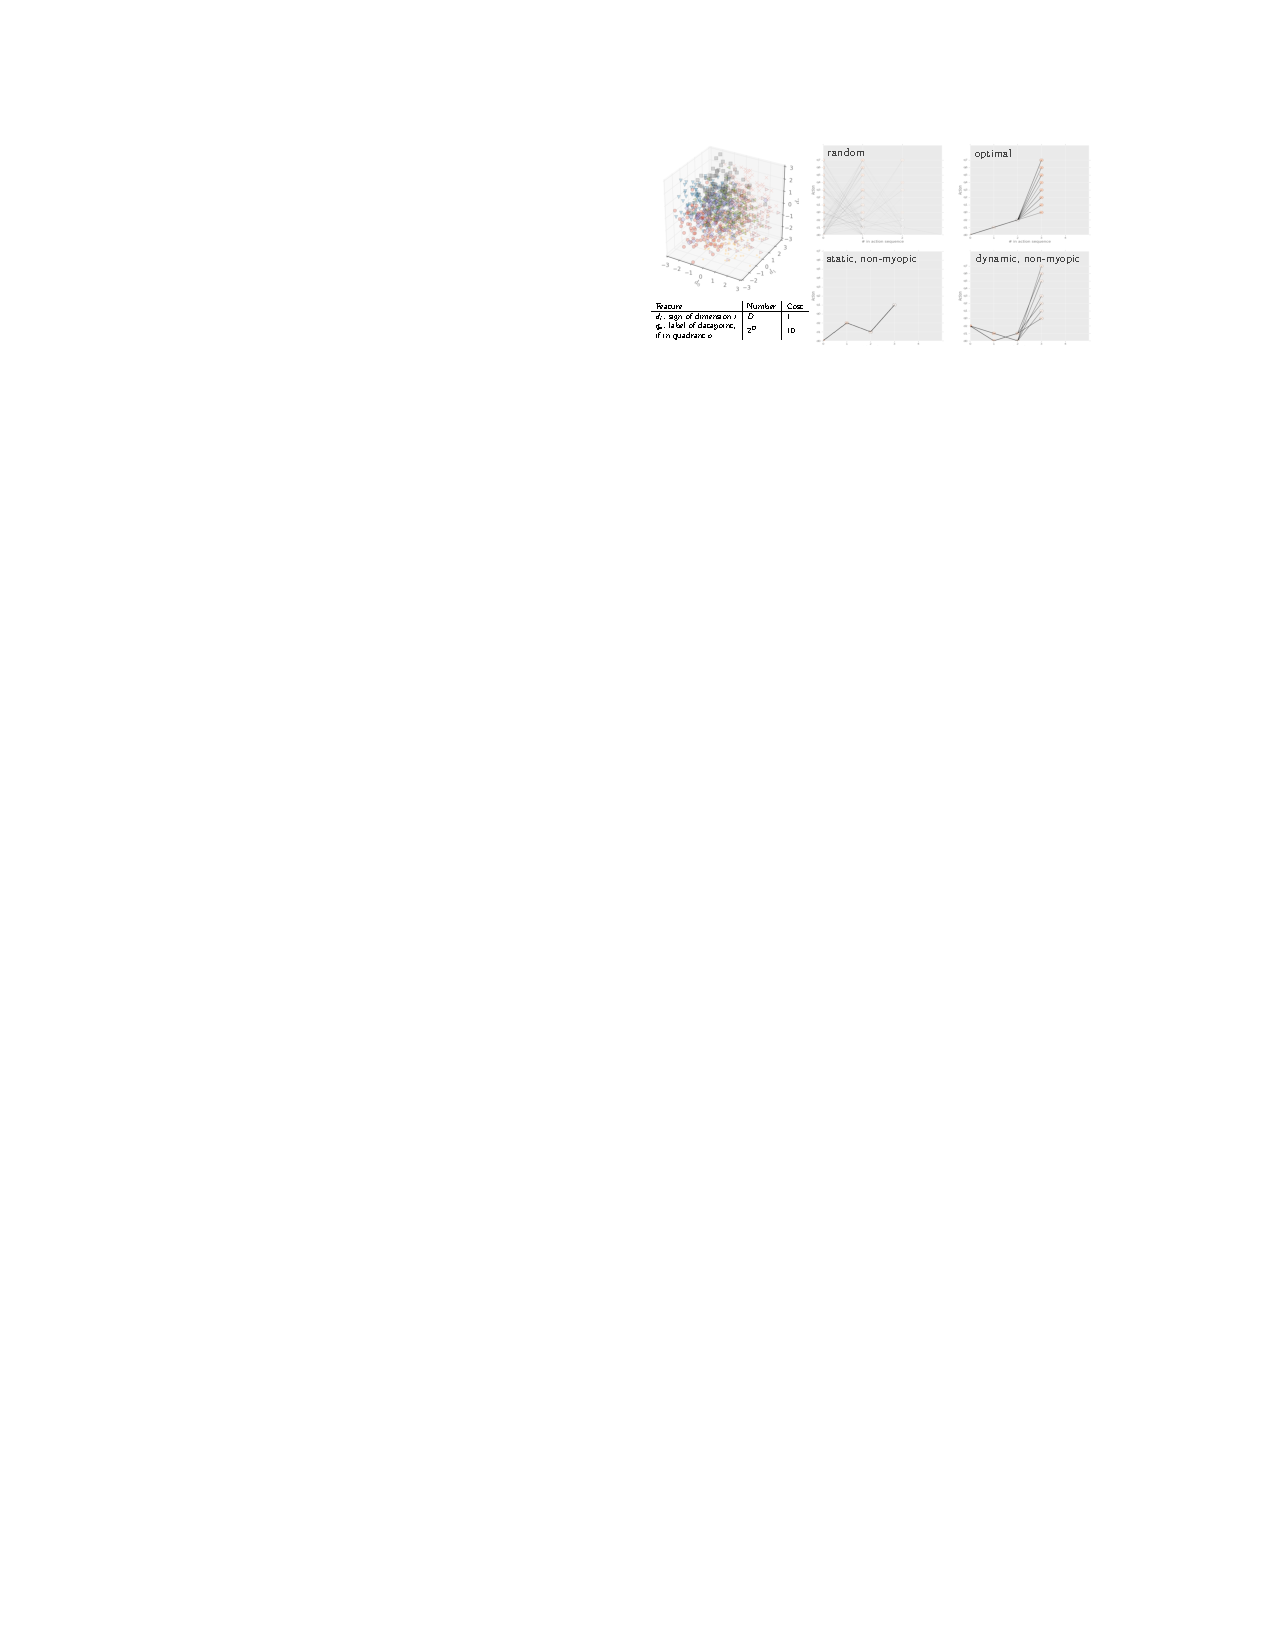
\includegraphics[width=0.8\linewidth]{../figures/my_cstc.pdf}
}
\end{frame}

\subsection[Adaptive Submod.]{Adaptive submodular functions}

\begin{frame}\frametitle{Adaptive submodularity}
\begin{itemize}
    \item Introduced by \cite{Golovin-and-Krause-2010-JAIR}\footnote{JAIR Best Paper Prize 2013}.
    \pause
    \item All $F$ potential observations $X_i$ are now random variables taking on values in $\mathcal{O}$, and have \emph{realization} $\mathbf{x}$.
    \pause
    \item Selected subset $\mathcal{X}_S \subseteq \mathcal{X}$ forms a \emph{partial realization} $\mathbf{x}_S$.
    \pause
    \item The objective function $f: 2^F \times |\mathcal{O}|^F \rightarrow \mathcal{R}$ takes a realization as well as the selected subset.
    \pause
    \item The \emph{policy} $\pi$ maps partial realizations to new observations, and can be thought of as a decision tree.
    \pause
    \item $F(\pi) = \mathbb{E}[f(\pi(\mathbf{x}), \mathbf{x})] = \sum_{\mathbf{x}} P(\mathbf{x}) f(\pi(\mathbf{x}), \mathbf{x})$
\end{itemize}
\centering
\visible<5->{
    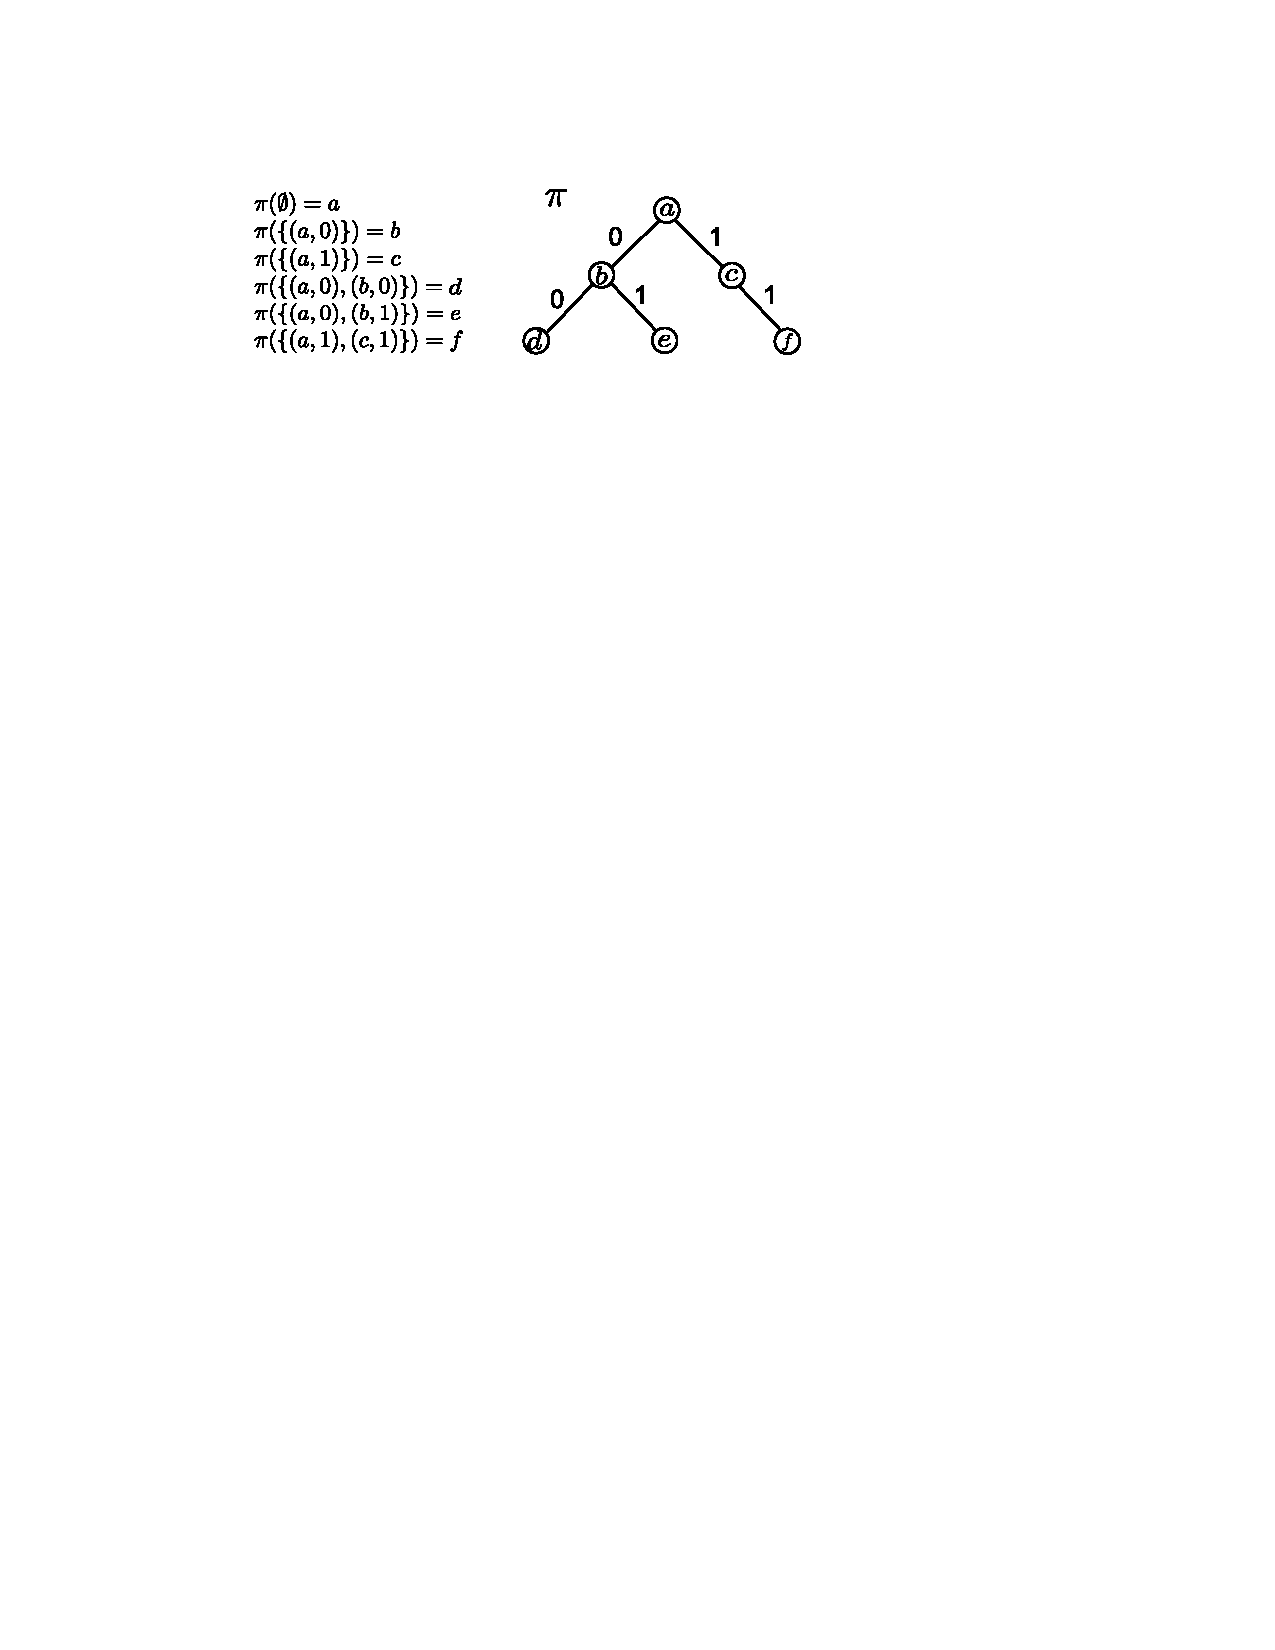
\includegraphics[width=.8\linewidth]{../figures/policy_and_tree.pdf}
}
\end{frame}

\begin{frame}\frametitle{Adaptive submodular functions}
\begin{itemize}
    \item We transfer the guarantees of greedy optimization with submodular functions to the adaptive setting by taking expectation over realizations, conditioned on the current partial realization.
    \pause
    \item Define the \emph{conditional expected gain} of adding another item to a set as
$$\Delta_f(X \mid \mathbf{x}_A) = \mathbb{E}\left[ f(\mathcal{X}_A \cup \{X\}, \mathbf{x}) - f(\mathcal{X}_A, \mathbf{x}) \mid \mathbf{x}_A \right]$$
    \pause
    \item For all $X$, the function must be adaptive submodular. %Observing an item with a smaller partial realization helps more than observing the same item with a larger partial realization.
$$\mathbf{x}_A \preceq \mathbf{x}_B \implies \Delta_f(X \mid \mathbf{x}_A) \geq \Delta_f(X \mid \mathbf{x}_B)$$
    \pause
    \item For all $X$, the function must be adaptive monotone.
$$\Delta_f(X \mid \mathbf{x}_A) \geq 0$$
\end{itemize}
\end{frame}

\begin{frame}\frametitle{Greedy policy}
\begin{algorithm}[H]
\KwIn{Budget $N$; observation set $\mathcal{X}$; $p(\mathbf{x})$; objective $f$.}
\KwOut{Set $\groundsubset \subseteq \groundset$ of size $N$}
\Begin{
$\groundsubset\leftarrow\emptyset$; $\mathbf{x_S} \leftarrow \emptyset$\;
\For{$i=1$ \KwTo $k$}{
    \lForEach{$\elem\in\groundset\setminus \groundsubset$}{compute $\Delta_f(\elem \mid \mathbf{x}_S)$}
    Select $X^* \in \underset{X}{\argmax} \frac{\Delta_f(\elem \mid \mathbf{x}_S)}{c(X)}$\;
    Set $\groundsubset \leftarrow \groundsubset \cup \{\elem^{*}\}$\;
    \lnl{1} Observe value $\mathbf{x}^*$ and update $\mathbf{x}_S \leftarrow \mathbf{x}_S \cup \mathbf{x}^*$\;
    }
}
\end{algorithm}
\end{frame}

\begin{frame}\frametitle{Submodularity $\rightarrow$ Adaptive submodularity}
Remarkably, optimality bounds stay the same!
\vspace{2em}

\begin{columns}[c]
\column{.45\linewidth}
\centering
\underline{Submodularity}
\tiny{
\begin{itemize}
    \item Works with sets.
    \item $\Delta_f(X \mid \mathcal{X}_A) = f(\mathcal{X}_A \cup \{X\}) - f(\mathcal{X}_A)$
    \item $\Delta_f(X \mid \mathcal{X}_A) \geq \Delta_f(X \mid \mathcal{X}_B)$ if $\mathcal{X}_A \subseteq \mathcal{X}_B$
    \item $\Delta_f(X \mid \mathcal{X}_A) \geq 0$
    \item $\underset{\mathcal{X}_S}{\max}\ f(\mathcal{X}_S)$ s.t. $|\mathcal{X}_S| \leq N$
    \item Budgeted maximization: greedy is within $(1 - 1/e)$ of OPT.
    \item Min-cost cover: greedy subset size is less than $1 + log \max_X f(X)$ of OPT subset size.
\end{itemize}
}

\column{.55\linewidth}
\centering
\underline{Adaptive submodularity}
\tiny{
\begin{itemize}
    \item Works with policies.
    \item $\Delta(X \mid \mathbf{x}_A) = \mathbb{E}\left[ f(\mathcal{X}_A \cup \{X\}, \mathbf{x}) - f(\mathcal{X}_A, \mathbf{x}) \mid \mathbf{x}_A \right]$
    \item $\Delta_f(X \mid \mathbf{x}_A) \geq \Delta_f(X \mid \mathbf{x}_B)$ if $\mathbf{x}_A \preceq \mathbf{x}_B$
    \item $\Delta_f(X \mid \mathbf{x}_A) \geq 0$
    \item $\underset{\pi}{\max}\ F(\pi)$  s.t. $|\pi| \leq N$
    \item Budgeted maximization: greedy policy is within $(1 - 1/e)$ of OPT policy.
    \item Min-cost cover: greedy policy size is less than $1 + log \max_X f(X,
    \mathbf{x})$ of OPT policy size.
\end{itemize}
}
\end{columns}
\end{frame}

\subsection{Additional benefits}

\begin{frame}\frametitle{Benefit: Lazy evaluation}
\begin{itemize}
    \item A neat algorithmic speed-up follows from the submodularity of the objective: \textbf{the expected utility of an observation cannot increase}. This means not all observations need to be evaluated on every iteration.
\end{itemize}
\vspace{2em}
\centering
\includegraphics<2>[width=0.8\linewidth]{../figures/lazy1.png}
\includegraphics<3>[width=0.8\linewidth]{../figures/lazy2.png}
\includegraphics<4>[width=0.8\linewidth]{../figures/lazy3.png}
\includegraphics<5>[width=0.8\linewidth]{../figures/lazy4.png}
\includegraphics<6>[width=0.8\linewidth]{../figures/lazy5.png}
\end{frame}

% \begin{frame}\frametitle{Benefit: Data-dependent bounds}
% \begin{itemize}
%     \item
% \end{itemize}
% \end{frame}


%% Active Classification
\section[Objective]{Formulating the objective}

\begin{frame}\frametitle{Formulating the objective}
\begin{itemize}
    \item So far, things look promising!
    \pause
    \item Unfortunately, infogain is only adaptive submodular in the noiseless setting (in Naive Bayes, only one outcome $\mathbf{x}_i$ given $h$).
    \pause
    \item If there is noise, need to find an objective that both optimizes what we want and is adaptive submodular.
    \pause
    \item Have two previously explored options:
    \begin{itemize}
        \item \emph{Hypothesis Pruning} [\cite{DBLP:journals/corr/abs-1010-3091}]
        \item \emph{Equivalence Class Edge Cutting} [\cite{DBLP:journals/corr/abs-1208-6067}]
    \end{itemize}
    \pause
    \item Both have proofs only for the Min-Cost Cover setting.
\end{itemize}
\end{frame}

\begin{frame}\frametitle{Hypothesis pruning}
\begin{itemize}
    \item Motivation: efficiently figure out where an object is in 3D space so that a robotic arm can grasp it.
    \pause
    \item Idea: downweight hypotheses with a non-normalized Gaussian, which effectively removes a portion of the hypothesis space. By construction, the probability mass of the posterior distribution can only become smaller with each step.
    \item Proof: lengthy (in report). Tricky to prove that the \emph{expected} utility does not increase.
\end{itemize}
\end{frame}

\begin{frame}\frametitle{Equivalence Class Edge Cutting}
\begin{itemize}
    \item Motivation: request most informative instance to be labeled by an oracle.
    \pause
    \item Idea: expand the space of realizations to account for all possible noise settings. A single hypothesis can now be true in multiple states. Find the test that removes the most hypotheses.
    \item Proof: lengthy (in report).
\end{itemize}
\visible<2->{
\centering
    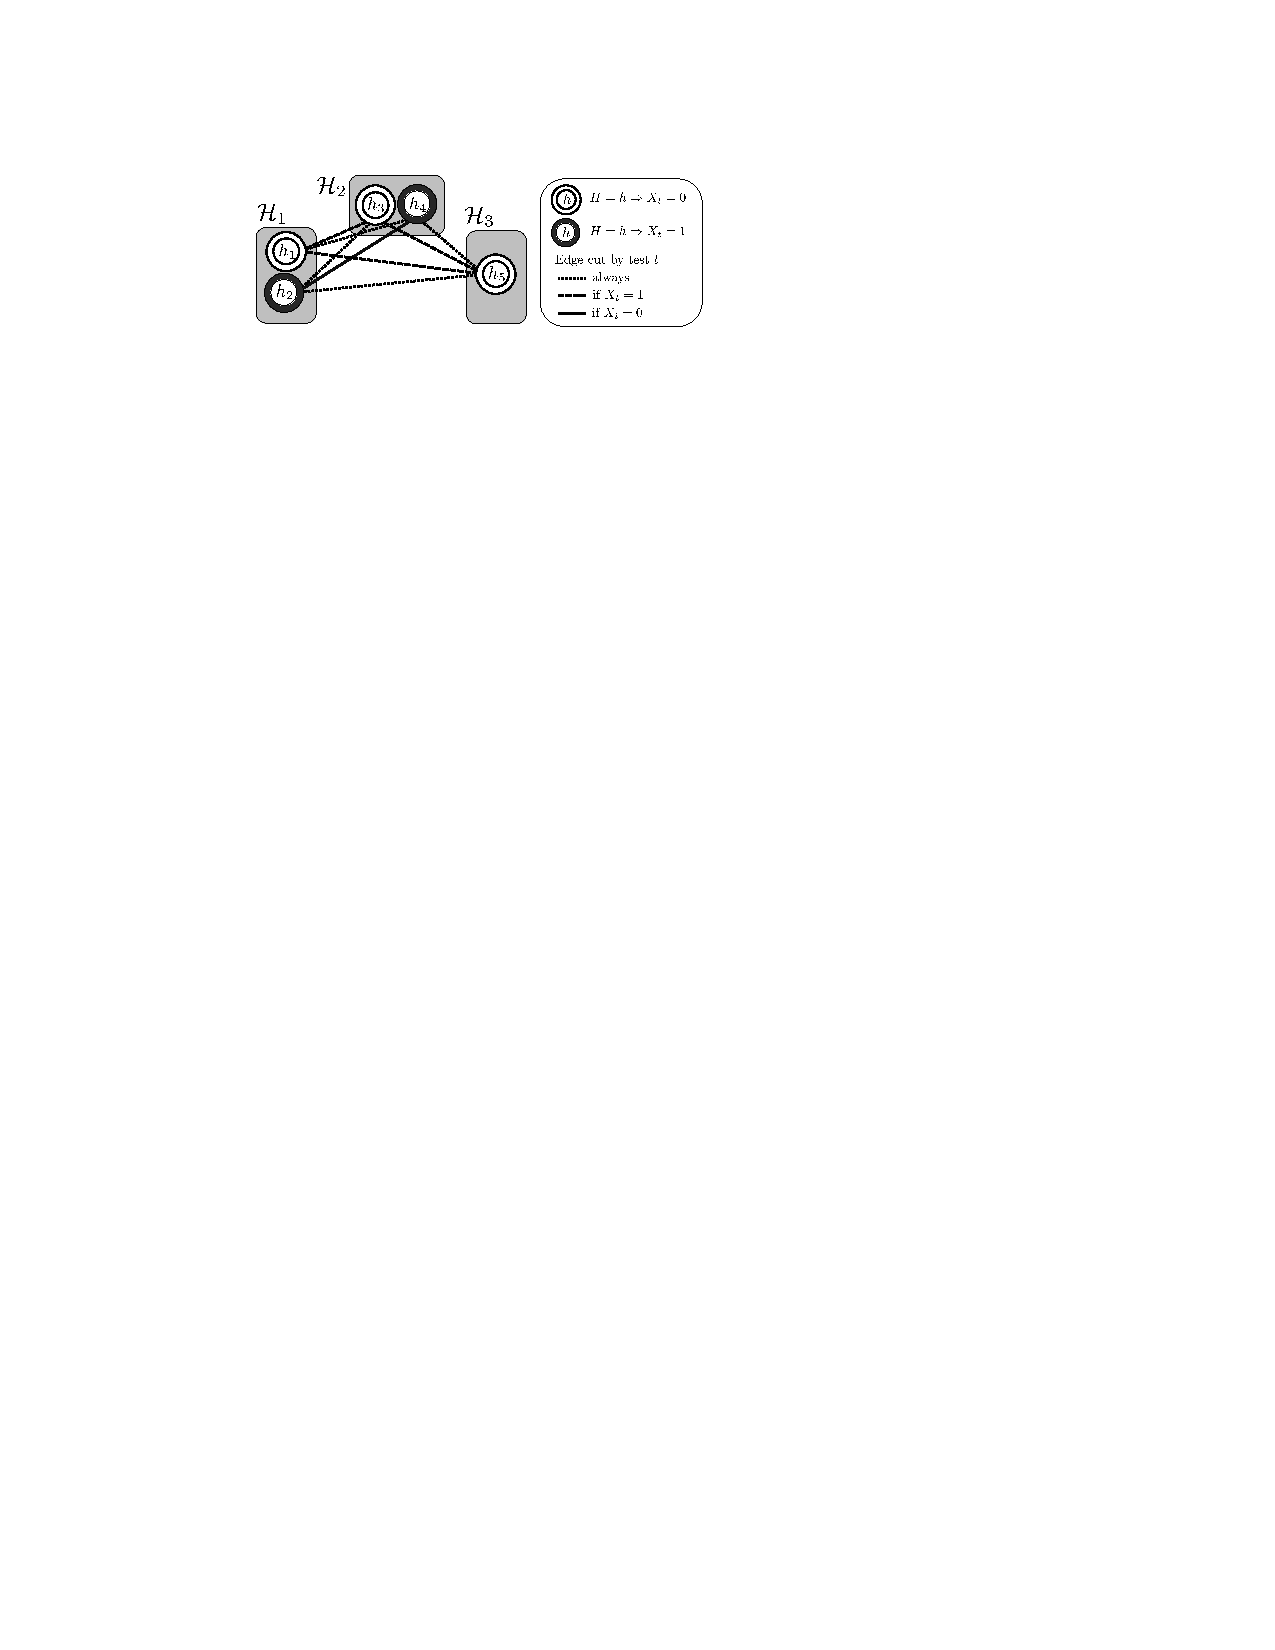
\includegraphics[width=.8\linewidth]{../figures/ecec.pdf}
}
\end{frame}


%% Future work
\section{Future work}

\begin{frame}\frametitle{Future Work}
\begin{itemize}
    \item Empirically evaluate the two adaptive submodular objectives against my current POMDP approach and on my datasets.
    \begin{itemize}
        \item Adaptive submodularity of a function can depend on the distribution $p(\mathbf{x})$.
    \end{itemize}
    \pause
    \item Modular\footnote{$c(\mathcal{X}_S) = \sum_{X \in \mathcal{X}_S} c(X)$} costs are fine. How about submodular costs?
    \pause
    \item Analyze the adaptivity gap of these methods via data-dependent bounds.
\end{itemize}
\end{frame}

%% References
\begin{frame}
\frametitle{References}
\small{\bibliography{../references}}
\end{frame}

\end{document}
